% Figure 1 -- study overview / pipeline.
% Vector TikZ source; compiled to results/figures/fig_pipeline.pdf by make_flowchart.py.
% Build manually with:  pdflatex fig_pipeline.tex
\documentclass[tikz,border=2pt]{standalone}
\usepackage[T1]{fontenc}
\usepackage{newtxtext,newtxmath}
\usetikzlibrary{arrows.meta,positioning,calc}

\definecolor{ink}{HTML}{1E222B}
\definecolor{sub}{HTML}{6E7480}
\definecolor{navy}{HTML}{2C4A73}
\definecolor{ngreen}{HTML}{1E7A5F}
\definecolor{nred}{HTML}{B23A2E}

\hyphenpenalty=10000
\exhyphenpenalty=10000

\newcommand{\dt}{\,$\cdot$\,}
\newcommand{\head}[2]{{\footnotesize\bfseries\color{#1}#2}}
\newcommand{\hnote}[1]{{\scriptsize\color{sub}#1}}

\begin{document}
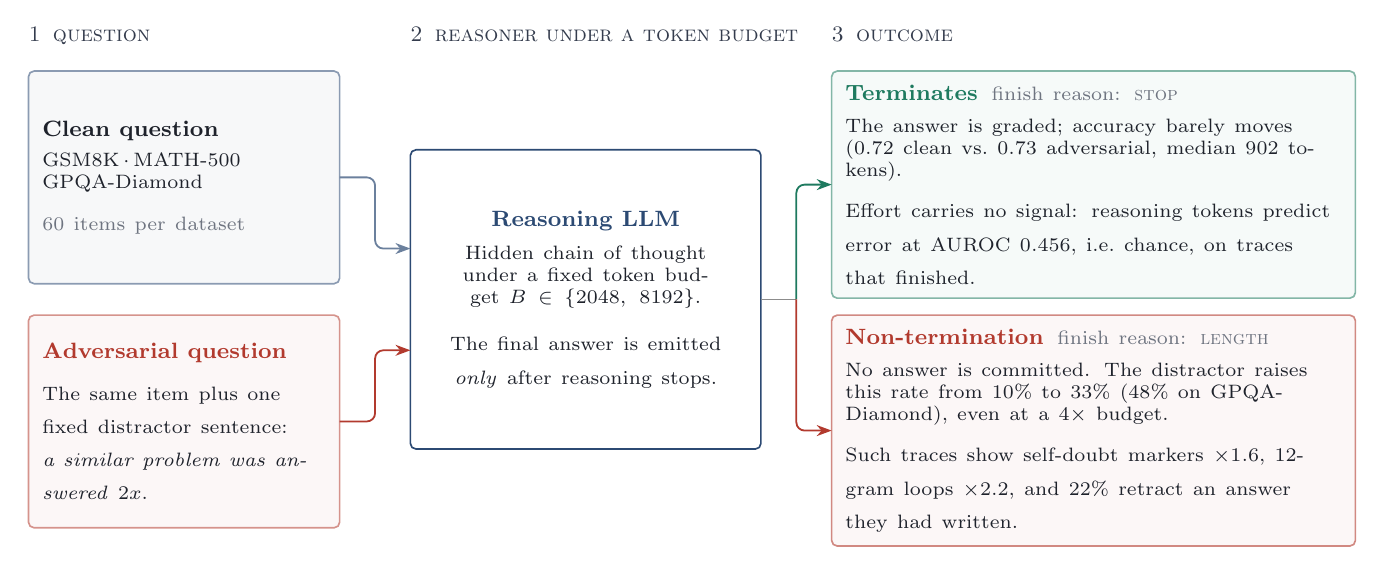
\begin{tikzpicture}[
  x=1cm, y=1cm,
  every node/.style={inner sep=0pt, outer sep=0pt, text=ink},
  box/.style={rounded corners=2pt, line width=0.6pt, draw=#1,
              align=left, inner sep=5pt, anchor=north west},
  flow/.style={-{Stealth[length=1.9mm,width=1.4mm]}, line width=0.65pt,
               rounded corners=3pt, color=#1},
  stage/.style={anchor=base west, font=\footnotesize\scshape, text=sub!140},
]

% ---------------------------------------------------------------- geometry
\def\rowa{4.85}   % top edge, row 1
\def\rowb{1.75}   % top edge, row 2
\def\rowh{2.70}   % row height
\def\xa{0}        % left column
\def\xb{4.85}     % middle column
\def\xc{10.20}     % right column

% ---------------------------------------------------------------- inputs
\node[box=navy!55, fill=navy!4, text width=3.6cm, minimum height=\rowh cm]
     (I1) at (\xa,\rowa)
  {\head{ink}{Clean question}\\[3pt]
   {\scriptsize GSM8K\dt MATH-500\\ GPQA-Diamond\\[3pt]
    \color{sub}60 items per dataset}};

\node[box=nred!55, fill=nred!4, text width=3.6cm, minimum height=\rowh cm]
     (I2) at (\xa,\rowb)
  {\head{nred}{Adversarial question}\\[3pt]
   {\scriptsize The same item plus one fixed distractor sentence:
    \emph{a similar problem was answered} $2x$.}};

% ---------------------------------------------------------------- reasoner
\node[box=navy, fill=white, text width=4.1cm, minimum height=3.8cm,
      align=center] (M) at (\xb,3.85)
  {\head{navy}{Reasoning LLM}\\[4pt]
   {\scriptsize Hidden chain of thought under a fixed token budget
    $B \in \{2048,\ 8192\}$.\\[5pt]
    The final answer is emitted \emph{only} after reasoning stops.}};

% ---------------------------------------------------------------- outcomes
\node[box=ngreen!55, fill=ngreen!4, text width=6.3cm, minimum height=\rowh cm]
     (O1) at (\xc,\rowa)
  {\head{ngreen}{Terminates}\enspace\hnote{finish reason: \textsc{stop}}\\[3.5pt]
   {\scriptsize The answer is graded; accuracy barely moves ($0.72$ clean
    vs.\ $0.73$ adversarial, median 902 tokens).\\[3pt]
    Effort carries no signal: reasoning tokens predict error at AUROC
    $0.456$, i.e.\ chance, on traces that finished.}};

\node[box=nred!60, fill=nred!4, text width=6.3cm, minimum height=\rowh cm]
     (O2) at (\xc,\rowb)
  {\head{nred}{Non-termination}\enspace\hnote{finish reason: \textsc{length}}\\[3.5pt]
   {\scriptsize No answer is committed. The distractor raises this rate from
    10\% to 33\% (48\% on GPQA-Diamond), even at a $4\times$ budget.\\[3pt]
    Such traces show self-doubt markers $\times 1.6$, 12-gram loops
    $\times 2.2$, and 22\% retract an answer they had written.}};

% ---------------------------------------------------------------- flow
\coordinate (jout) at ($(M.east) + (0.45,0)$);

\draw[flow=navy!70] (I1.east) -- ++(0.45,0) |- ($(M.north west)!0.33!(M.south west)$);
\draw[flow=nred]    (I2.east) -- ++(0.45,0) |- ($(M.north west)!0.67!(M.south west)$);
\draw[line width=0.65pt, color=black!45] (M.east) -- (jout);
\draw[flow=ngreen] (jout) |- (O1.west);
\draw[flow=nred]   (jout) |- (O2.west);

% ---------------------------------------------------------------- stages
\node[stage] at (\xa,5.22) {1\enspace question};
\node[stage] at (\xb,5.22) {2\enspace reasoner under a token budget};
\node[stage] at (\xc,5.22) {3\enspace outcome};

\end{tikzpicture}
\end{document}
